\documentclass[11pt]{book}
\usepackage[utf8]{vietnam}
\usepackage{amsmath,amsxtra,amssymb,latexsym, amscd,amsthm}
\usepackage{graphicx}
\usepackage{picinpar}
\usepackage{mathrsfs}
\usepackage{tikz}
%\usepackage{tikz-3dplot-circleofsphere}
\usetikzlibrary{calc,patterns,intersections,angles,arrows,matrix,quotes,patterns}
%\usepackage{tkz-euclide}
\usepackage{tkz-tab}
%\usepackage{tabvar}
\usepackage{tkz-base}
\usepackage{longtable}%
\usepackage[colorlinks,hyperindex,plainpages=false,unicode]{hyperref}
\usepackage{calc}
\usepackage{mathpazo} 
\def\dx{\mathrm{\, d}x}
%%%%%%%%%\hoffset=-2.8cm
\voffset=-2.5cm
\textheight 25truecm 
\textwidth 19truecm 
%  \usepackage[paperwidth=16truecm,paperheight=24truecm]{geometry}
% \textheight 19.5truecm %%16.2truecm 
% \textwidth 12 truecm 
\parskip 3pt
\headsep=12pt
\usepackage[baitap]{dethi}

\tentruong{NHÓM VẼ HÌNH KHOA HỌC}
\tenkhoa{\underline{TIKZ-ASYMPTOTE}}
\madethi{104} 
\loaidethi{(Đề gồm  0\pageref{dbPage} trang)}

\tenkythi{ĐỀ KIỂM TRA MẪU VỚI GÓI DETHI}
\namhoc{Năm: 2021}
\tenmonhoc{Môn: LaTeX - TikZ}
\thoigian{\underline{Thời gian làm bài: 90 phút, không kể thời gian giao đề}}   
%\tieudetrenbaitap{Bùi Quỹ - Trung tâm GDNN-GDTX Duy Tiên}
%\tieudeduoibaitap{LaTeX - TikZ - năm 2021}

\trangcuoi{dbPage}
\hovaten{Họ và tên}         %Nếu không muốn có dòng này không gõ lệnh
% \tenlop{Tên lớp}         %Nếu không muốn có dòng này không gõ lệnh
\sobaodanh{Số báo danh}  %Nếu không muốn có dòng này không gõ lệnh
%\khoanhd{\cboxv}{}
\daungoac{\cboxx}{}
\chuphuongan{\small\bfseries\Alph}
\mauchu{blue}
\chucauhoi{Bài}
\chuloigiai{Hướng dẫn:}
\PSNrandseed{\time}
\parindent 10pt
%\graphicspath{{hinh-duan07/}{temp/}}
% \nguondetrue
\duongkefalse
\usepackage{nonfloat}
\setlength{\baselineskip}{12truept}
\def\v#1{\overrightarrow{#1}} %Làm vectơ
\everymath{\displaystyle}
\def\cung#1{\stackrel\frown{#1}}

\usepackage{times}
\fontsize{13pt}{13pt}\selectfont
\begin{document}
	%\soanthao
	%%%%%%%%%%%%%
	%\loadallproblems[tnhamso]{Data/tnhamso}
	%\loadallproblems[tnsophuc]{Data/tnsophuc}
	%\loadallproblems[tuluan]{Data/tuluan}
	%\loadallproblems[chontu]{Data/tnchontu}
	%\loadallproblems[gachduoi]{Data/gachduoi}
	%\loadallproblems[dungsai]{Data/dung-sai}
	%\loadallproblems[dienchotrong]{Data/dienchotrong}
	%%%%%%%%
	%\loadrandomproblems[104]{8}{Data/tracnghiem}
	%\loadrandomproblems[105]{5}{Data/Hanam2021-104}
	%\loadrandomproblems[106]{5}{Data/tnhamso}
	%\loadrandomproblems[107]{5}{Data/tnhamso}
	%\loadrandomproblems[tnsophuc]{5}{Data/tnsophuc}
	%\loadrandomproblems[tuluan]{5}{Data/tuluan}
	%\loadrandomproblems[chontu]{5}{Data/tnchontu}
	%\loadrandomproblems[gachduoi]{5}{Data/gachduoi}
	%\loadrandomproblems[dungsai]{5}{Data/dung-sai}
	%\loadrandomproblems[dienchotrong]{5}{Data/dienchotrong}
	%%%%%%%%%%%%%%%%%
	%\indebai
	\lamtieudetracnghiem
	\soanthao
	\indebai
	\indebailoigiai
	
	%\indebaima{104}
	%\indebaima{105}
	
	%%%%%%%%%%%%%%%%%%%%%
	%%%%%%%%%%%%%%%%%%%%%%%%
	\lamtieude
	\noindent{\bfseries Mẫu câu hỏi}
	\baitracnghiem{VDTN:02}{
	Nội dung câu hỏi trắc nghiệm
}{
	\bonpa{1}%Phương án 1 là đúng
	{Phương án 1.}
	{Phương án 2.}
	{Phương án 3.}
	{Phương án 4.}
}{
	Nội dung lời giải chi tiết.
}
\baitndungsai{VDDS:03}{
	Nội dung câu hỏi đúng sai.
}{\bonpads[1] %Đảo hai phương án 2 và 3
	{\dungsai{\dsdung}{Phương án 1.}}
	{\dungsai{\dssai}{Phương án 2.}}
	{\dungsai{\dsdung}{Phương án 3.}}
	{\dungsai{\dssai}{Phương án 4.}}
}{
	Nội dung lời giải chi tiết.
}

\baitndungsai{VDDS:04}{
	Nội dung câu hỏi đúng sai nhiều phương án.
}{\phuongands%Số phương án tùy ý (không xáo trộn các phương án khi biên dịch)
	\dungsai{\dsdung}{Phương án 1.}
	\dungsai{\dssai}{Phương án 2.}
	\dungsai{\dsdung}{Phương án 3.}
	\dungsai{\dssai}{Phương án 4.}
	\dungsai{\dssai}{Phương án 5.}
	\dungsai{\dsdung}{Phương án 6.}
}{
	Nội dung lời giải chi tiết.
}

\baitraloingan{VDTLN:02}{
	Nội dung câu hỏi trả lời ngắn.
}{
	\dapantln{0}{,}{0}{1}
}{
	Nội dung lời giải chi tiết.
}
\baituluan{VDTL:02}{
	Nội dung câu hỏi tự luận.
}{
	Nội dung lời giải chi tiết
}

	
	\noindent\textbf{Phần I. Nhiều phương án lựa chọn}
	\setcounter{question}{0}
	\baitracnghiem{De01TNKQ:01}{
	Trong không gian $Oxyz$, hình chiếu vuông góc của điểm $M(-2;0;1)$ lên trục $Oy$ có tọa độ là:
}{
	\bonpa{1}
	{$(0;0;0)$.}
	{$(-2;0;0)$.}
	{$(-2;0;1)$.}
	{$(0;0;1)$;}
}{
	
}

\baitracnghiem{De01TNKQ:02}{
	Hàm số nào dưới đây luôn nghịch biến trên $\mathbb{R}$?
}{
	\bonpa{3}
	{$y=\frac{x^{2}+x+3}{x+2}$.}
	{$y=\frac{2x-2}{x+1}$.}
	{$y=3-2x-x^{3}$.}
	{$y=x^{3}+x+1$.}
}{
	
}

\baitracnghiem{De01TNKQ:03}{
	Cho hình hộp $ABCD.A'B'C'D'$. Tìm véc tơ $\overrightarrow{u}=\overrightarrow{AB}+\overrightarrow{AD}+\overrightarrow{CC'}$.
}{
	\bonpa{2}
	{$\overrightarrow{u}=\overrightarrow{AC}$.}
	{$\overrightarrow{u}=\overrightarrow{AC'}$.}
	{$\overrightarrow{u}=\overrightarrow{A'C}$.}
	{$\overrightarrow{u}=\overrightarrow{C'A}$.}
}{
	
}

\baitracnghiem{De01TNKQ:04}{
	Tìm điểm cực tiểu của đồ thị hàm số $y=\frac{1}{3}x^{3}-2x^{2}+3x+1$.
}{
	\bonpa{2}
	{$x=1$.}
	{$\left(1;\frac{7}{3}\right)$.}
	{$x=3$.}
	{$(3;1)$.}
}{
	
}

\baitracnghiem{De01TNKQ:05}{
	Cho hàm số $y=f(x)$ có bảng biến thiên như hình dưới. 
	
	\centerline{
		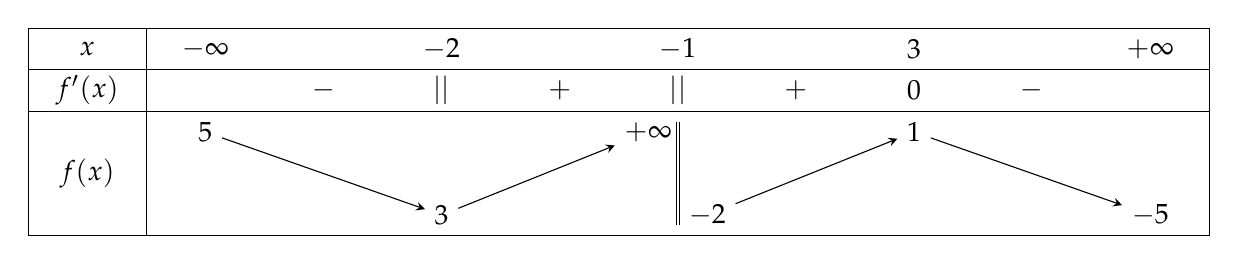
\begin{tikzpicture}[x=1.5cm,y=1.5em]
			\foreach \x/\gt in {0/x,1/-\infty,3/-2,5/-1,7/3,9/+\infty}\path (\x,0) node{$\gt$};
			\foreach \x/\gt in {0/f'(x),2/-,3/||,4/+,5/||,6/+,7/0,8/-}\path (\x,-1) node{$\gt$};
			\foreach \x/\y/\gt[count=\i from 0] in {0/-3/f(x),1/-2/5,3/-4/3,4.75/-2/+\infty,5.25/-4/-2,7/-2/1,9/-4/-5}\path (\x,\y) node(\i){$\gt$};
			\foreach \x/\y in {1/2,2/3,4/5,5/6}\draw[-stealth] (\x)--(\y);
			\draw (-.5,.5) rectangle (9.5,-4.5) (.5,.5)--(.5,-4.5) (-.5,-.5)--(9.5,-.5) (-.5,-1.5)--(9.5,-1.5);
			\draw[double] (5,-1.75)--(5,-4.25);
		\end{tikzpicture}
	}
	
	Đồ thị hàm số đã cho có tiệm cận đứng là:
}{
	\bonpa{1}
	{$x=-1$.}
	{$x=-2$.}
	{$y=1$.}
	{$y=5$.}
}{
	
}

\baitracnghiem{De01TNKQ:06}{
	Đường cong trong hình dưới đây là đồ thị của hàm số nào?
	
	\centerline{
		\begin{tikzpicture}
			\draw[-stealth] (-3,0)--(2,0) node[below]{$x$};
			\draw[-stealth] (0,-2.5)--(0,3) node[left]{$y$};
			\clip (-3,-2.5) rectangle (3,2);
			\draw[dashed] (-2,0) node[below]{$-2$}|-(0,2) node[right]{$2$};
			\draw[smooth] plot[domain=-3:3] (\x,{(\x)^3+3*(\x)^2-2});
			\path 
			(0,0) node[above left]{$O$}
			(-1,0) node[below]{$-1$}
			(0,-2) node[left]{$-2$}
			;
		\end{tikzpicture}
	}
	
}{
	\bonpa{2}
	{$y=-x^{3}-3x^{2}-2$.}
	{$y=x^{3}+3x^{2}-2$.}
	{$y=x^{3}-3x^{2}-2$.}
	{$y=-x^{3}+3x^{2}-2$.}
}{
	
}

\baitracnghiem{$De01TNKQ:07$}{
	Đường thẳng $x=-1$ là tiệm cận đứng của hàm số nào sau đây?
}{
	\bonpa{3}
	{$y=\frac{x+1}{x^{2}+4x+3}$.}
	{$y=\frac{x+1}{x^{2}+1}$.}
	{$y=\frac{x^{2}-3x+2}{x^{2}-1}$.}
	{$y=\frac{x^{2}+3x+2}{x^{2}-1}$.}
}{
	
}

\baitracnghiem{De01TNKQ:08}{
	Giá trị lớn nhất của hàm số $f(x)=\frac{3x-1}{x-3}$ trên $[0;2]$ là:
}{
	\bonpa{2}
	{$M=5$.}
	{$M=\frac{1}{3}$.}
	{$M=-5$.}
	{$M=-\frac{1}{3}$.}
}{
	
}

\baitracnghiem{De01TNKQ:09}{
	Gọi $A$ là giao điểm của đồ thị hàm số $y=\frac{x-2}{2x+1}$ với trục $Ox$. Giá trị đạo hàm của hàm số đã cho tại điểm $A$ là:
}{
	\bonpa{4}
	{$-\frac{5}{9}$.}
	{$-\frac{1}{3}$.}
	{$\frac{5}{9}$.}
	{$\frac{1}{3}$.}
}{
	
}

\baitracnghiem{De01TNKQ:10}{
	Cho lăng trụ đều $ABC.A'B'C'$. Góc giữa $\overrightarrow{BA}$ và $\overrightarrow{C'B'}$ bằng:
}{
	\bonpa{3}
	{$30^{\circ}$.}
	{$60^{\circ}$.}
	{$120^{\circ}$.}
	{$90^{\circ}$.}
}{
	
}

\baitracnghiem{De01TNKQ:11}{
	Trong không gian $Oxyz$. Cho điểm $M$ thỏa mãn $\overrightarrow{OM}=2\overrightarrow{i}-\overrightarrow{k}$. Khi đó tọa độ của điểm $M$ là:
}{
	\bonpa{2}
	{$(2;-1;0)$.}
	{$(2;0;-1)$.}
	{$(0;2;-1)$.}
	{$(-2;0;1)$.}
}{
	
}

\baitracnghiem{De01TNKQ:12}{
	Hàm số $f(x)=x^{3}-3x^{2}+1$ đạt cực đại tại:
}{
	\bonpa{4}
	{$x=2$.}
	{$y=2$.}
	{$y=0$.}
	{$x=0$.}
}{
	
}

\baitracnghiem{De01TNKQ:13}{
	Cho hàm số $f(x)$ có bảng biến thiên như sau:
	
	\centerline{
		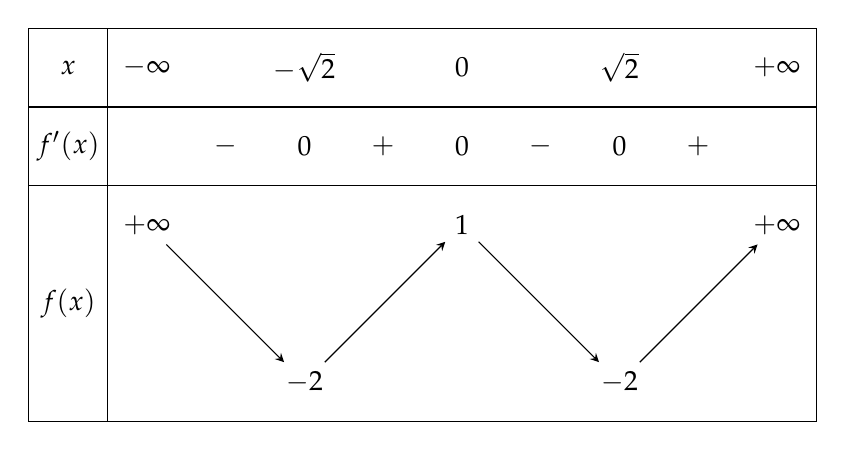
\begin{tikzpicture}
			\foreach \x/\gt in {0/x,1/-\infty,3/-\sqrt{2},5/0,7/\sqrt{2},9/+\infty}\path (\x,0) node{$\gt$};
			\foreach \x/\gt in {0/f'(x),2/-,3/0,4/+,5/0,6/-,7/0,8/+}\path (\x,-1) node{$\gt$};
			\foreach \x/\y/\gt[count=\i from 0] in {0/-3/f(x),1/-2/+\infty,3/-4/-2,5/-2/1,7/-4/-2,9/-2/+\infty}\path (\x,\y) node(\i){$\gt$};
			\foreach \x/\y in {1/2,2/3,3/4,4/5}\draw[-stealth] (\x)--(\y);
			\draw (-.5,.5) rectangle (9.5,-4.5) (.5,.5)--(.5,-4.5) (-.5,-.5)--(9.5,-.5) (-.5,-1.5)--(9.5,-1.5); 
		\end{tikzpicture}
	}
	
	Hàm số $f(x)$ nghịch biến trên khoảng nào?
}{
	\bonpa{2}
	{$(-\sqrt{2};\sqrt{2})$.}
	{$(-\infty;-\sqrt{2})$.}
	{$(-\sqrt{2};0)$.}
	{$(\sqrt{2};+\infty)$.}
}{
	
}

\baitracnghiem{De01TNKQ:14}{
	Hàm số $f(x)=\sqrt{x^{2}-2x}$ nghịch biến trên khoảng nào sau đây?
}{
	\bonpa{3}
	{$(2;+\infty)$.}
	{$(0,2)$.}
	{$(-\infty;0)$.}
	{$\mathbb{R}$.}
}{
	
}
%%10:59:48 10/11/2024Last Modification of contents
	\noindent\textbf{Phần II. Trắc nghiệm đúng sai}
	\setcounter{question}{0}
	\baitndungsai{De01DS:01}{
	Trong không gian $Oxyz$, cho ba điểm $A(2;-1;1)$, $B(-1;3;-1)$ và $\overrightarrow{u}=(1;2;3)$. Xét tính đúng, sai của các khẳng định sau:
}{\bonpatest
	{\TFTrue Tọa độ véc tơ $\overrightarrow{AB}$ là $(-3;4;-2)$.}
	{Tọa độ điểm $C$ để $\overrightarrow{AC}=\overrightarrow{u}$ là $(3;3;4)$}
	{Tọa độ trung điểm $I$ của $AC$ là $(5;0;5)$.}
	{\TFTrue Tọa độ điểm $D$ để $ABCD$ là hình bình hành là $(6,-3,6)$.}
}{
	Nội dung lời giải
}

\baitndungsai{De01DS:02}{
	Cho hàm số $y=\frac{-x^{2}-3x+4}{x-3}$ có đồ thị $(C)$. Xét tính đúng sai của các mệnh đề sau:
}{\bonpatest
	{\TFTrue Đồ thị $(C)$ có đường tiệm cận xiên là $y=-x-6$.}
	{\TFTrue Đồ thị $(C)$ nhận điểm $I(3;-9)$ làm tâm đối xứng.}
	{Hàm số $y=f(x)$ đã cho đồng biến trên $(3;7)$.}
	{\TFTrue Đồ thị $(C)$ có hai điểm cực trị nằm ở hai phía đối với trục $Oy$.}
}{
	
}

\baitndungsai{De01DS:03}{
	Cho hàm số $f(x)=\frac{2x^{3}+3x+7}{x-1}$. Xét tính đúng sai của các khẳng định sau:
}{\bonpatest
	{$\lim\limits_{x\to -1^{+}}f(x)=-\infty$.}
	{\TFTrue Đường thẳng $x=-1$ là đường tiệm cận đứng của đồ thị hàm số.}
	{\TFTrue $\lim\limits_{x\to -\infty}\frac{f(x)}{x}=2$.}
	{\TFTrue Đường thẳng $y=2x+1$ là tiệm cận xiên của đồ thị hàm số.}
}{
	
}

\baitndungsai{De01DS:04}{
	Cho hàm số $f(x)=\sqrt{1-x}+\sqrt{1+x}$. Xét tính đúng sai của các khẳng định sau:
}{\bonpatest
	{\TFTrue Tập xác định của hàm số đã cho là $\mathbb{D}=[-1;1]$.}
	{Đạo hàm của hàm số đã cho là $f'(x)=\frac{\sqrt{1-x}-\sqrt{1+x}}{2\sqrt{1-x^{2}}}$ với mọi $x\in (-1;1)$.}
	{$\min\limits_{[-1;1]}f(x)=f(0)$.}
	{$\min\limits_{[-1;1]}f(x)+\max\limits_{[-1;1]}=2$.}
}{
	
}

\baitndungsai{De01DS:05}{
	Cho hàm số $y=f(x)$ xác định liên tục trên $\mathbb{R}$ và có bảng xét dấu đạo hàm như sau:
	
	\centerline{
		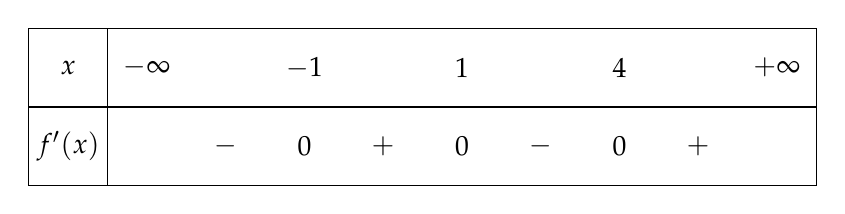
\begin{tikzpicture}
			\foreach \x/\gt in {0/x,1/-\infty,3/-1,5/1,7/4,9/+\infty}\path (\x,0) node{$\gt$};
			\foreach \x/\gt in {0/f'(x),2/-,3/0,4/+,5/0,6/-,7/0,8/+}\path (\x,-1) node{$\gt$};
			\draw (-.5,.5) rectangle (9.5,-1.5) (-.5,-.5)--(9.5,-.5) (.5,.5)--(.5,-1.5);
		\end{tikzpicture}
	}
	
	Xét tính đúng, sai của các khẳng định sau:
}{\bonpatest
	{\TFTrue Hàm số đã cho đồng biến trên các khoảng $(-1;1)$ và $(4;+\infty)$.}
	{Hàm số đạt cực đại tại $x=4$.}
	{\TFTrue $f'(x)=0\Rightarrow \left[\begin{array}{l} x=-1 \\ x=1 \\ x=4\end{array}\right.$.}
	{\TFTrue Hàm số đã cho có $2$ điểm cực tiểu.}
}{
	
}

\baitndungsai{De01DS:06}{
	Cho hình chóp $S.ABCD$ có đáy $ABCD$ là hình chữ nhật, cạnh bên $SA$ vuông góc với mặt phẳng đáy. Gọi $I$ là giao điểm của $AC$ và $BD$ Các khẳng định sau đúng hay sai?
}{\bonpatest
	{\TFTrue $\overrightarrow{SA}+\overrightarrow{SC}=2\overrightarrow{SI}$.}
	{\TFTrue $\overrightarrow{BC}\cdot\overrightarrow{SC}=\overrightarrow{AC}\cdot\overrightarrow{BC}$.}
	{$\overrightarrow{SA}+\overrightarrow{SC}=\overrightarrow{SB}+\overrightarrow{SD}$.}
	{$\overrightarrow{SA}-\overrightarrow{SI}=\overrightarrow{SI}-\overrightarrow{SB}$.}
}{
	
}

\baitndungsai{De01DS:07}{
	Một vật được ném ngang từ độ cao $4$ mét chuyển động theo hình dạng parabol có phương trình $h(t)=-at^{2}+4$  trong đó $t$ là thời gian (tính bằng giây), $h(t)$ là độ cao của vật tại thời gian $t$ (tính bằng mét). Biết  rằng tính từ thời gian vật bắt đầu chuyển động đến khi vật chạm đất là $4$ giây. Xét tính đúng sai của các khẳng định sau:
}{\bonpatest
	{\TFTrue Giá trị của hệ số $a$ là $a=\frac{1}{4}$.}
	{\TFTrue Tốc độ của vật tại thời điểm $t=2$ (giây) là $1$ ($m/s$).}
	{\TFTrue Tại thời điểm $t=2$ (giây) vật có độ cao là $h=2$ (mét).}
	{Nếu cùng lực ném ban đầu và nâng độ cao lên $8$ mét thì sau $4$ giây vật vẫn chạm đất.}
}{
	
}




	\noindent\textbf{Phần III. Trả lời ngắn}
	\setcounter{question}{0}
	\baitraloingan{De01TLN:01}{
	Cho hàm số $f(x)=x-3+\frac{1}{x-2}$. Tìm giá trị nhỏ nhất của hàm số đã cho trên $(2;+\infty)$.
}{
	\dapantln{1}{}{}{}
}{
	{\bfseries Lời giải:}
	
	Xét hàm số $f(x)=x-3+\frac{1}{x-2}$ trên $(2;+\infty)$.
	
	$f'(x)=1-\frac{1}{(x-2)^{2}}=0\Rightarrow x=3\in (2;+\infty)$. Ta có bảng biến thiên của hàm số trên $(2;+\infty)$ như sau:
	
	\centerline{
		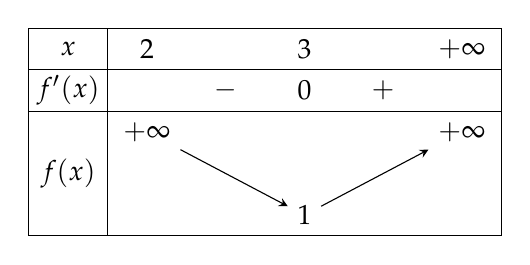
\begin{tikzpicture}[y=1.5em]
			\foreach \x/\gt in {0/x,1/2,3/3,5/+\infty}\path (\x,0) node{$\gt$};
			\foreach \x/\gt in {0/f'(x), 2/-,3/0,4/+}\path (\x,-1) node{$\gt$};
			\foreach \x/\y/\gt[count=\i from 0] in {0/-3/f(x),1/-2/+\infty,3/-4/1,5/-2/+\infty}\path (\x,\y) node(\i){$\gt$};
			\foreach \x/\y in {1/2,2/3}\draw[-stealth] (\x)--(\y);
			\draw (-.5,.5) rectangle (5.5,-4.5) (-.5,-.5)--(5.5,-.5) (-.5,-1.5)--(5.5,-1.5) (.5,.5)--(.5,-4.5);
		\end{tikzpicture}
	}
	
	Từ bảng biến thiên suy ra giá trị nhỏ nhất của hàm số $f(x)$ là $f(3)=1$.
}

\baitraloingan{De01TLN:02}{
	Cho hàm số $f(x)=x^{3}+3x^{2}-1$. Đồ thị hàm số có các điểm cạc đại, cực tiểu lần lượt là $A$ và $B$. Tính độ dài đoạn thẳng $AB$.
}{
	\dapantln{4}{,}{4}{7}
}{
	Hàm số $f(x)$ có đạo hàm $f'(x)=3x^{2}+6x$. $f'(x)$ có hai nghiệm $x=0$ và $x=-2$. Tương ứng các điểm $A(0;-1)$ và $B(-2;3)$.
	
	Do đó $AB=\sqrt{(-2-0)^{2}+(3-(-1))^{2}}=\sqrt{20}\simeq 4,47$.
}

\baitraloingan{De01TLN:03}{
	Một bác nông dân có mảnh vườn hình chữ nhật với chiều sâu $50$ mét, chiều rộng $20$ mét và $60$ mét lưới. Bác dự định căng lưới làm hàng rào để nuôi gà, lợi dụng một mặt tường bao dài $50$ mét nên bác chỉ cần căng lưới ba chiều còn lại. Tính diện tích lớn nhất mà bác nông dân có thể nuôi gà (tham khảo hình vẽ dưới đây)
	
	\centerline{
		\begin{tikzpicture}
			\draw[dashed] (0,5)--(0,0) node[pos=.5,left]{$50$ (m)}--(2,0) node[pos=.5,below]{$20$ (m)}--(2,5)--cycle; 
			\draw (0,5)--(1.5,5)--(1.5,3.5)--(0,3.5);
			\draw[-stealth] (1.5,4)--++(0:2) node[right]{lưới};
		\end{tikzpicture}
	}
}{
	\dapantln{2}{0}{0}{}
}{
	
}

\baitraloingan{De01TLN:04}{
	Sau khi đăng quang cuộc thi hoa hậu hoàn vũ Việt Nam năm 2024, một nhóm người
	đẹp đi làm từ thiện gồm có Hoa hậu, Á hậu 1 và Á hậu 2. Biết rằng nhóm sẽ không đi làm từ
	thiện nếu Hoa hậu rời nhóm hoặc cả hai Á hậu cùng rời nhóm. Khả năng để Hoa hậu, Á hậu
	1, Á hậu 2 rời nhóm lần lượt là $\frac{1}{4}$; $\frac{1}{5}$ và $\frac{3}{10}$. Biết các quyết định rời nhóm của Hoa hậu và các Á hậu độc lập nhau. Xác suất để nhóm có thể đi làm từ thiện bằng bao nhiêu?
}{
	\dapantln{0}{,}{7}{1}
}{
	{\bfseries Lời giải}
	
	Gọi $A$ là biến cố: Nhóm có thể đi làm từ thiện.
	
	$A_{1}$ là biến cố : Hoa hậu rời nhóm; $A_{2}$ là biến cố: Á hậu 1 rời nhóm; $A_{3}$ là biến cố: Á hậu 2 rời nhóm.
	
	Ta có: $A=\overline{A_{1}A_{2}A_{3}}\cup \overline{A_{1}}A_{2}\overline{A_{3}}\cup \overline{A_{1}}\overline{A_{2}}A_{3}$.
	
	Khi đó $P(A)=\frac{3}{4}\cdot \frac{4}{5}\cdot\frac{7}{10}+\frac{3}{4}\cdot\frac{1}{5}\cdot\frac{7}{10}+\frac{3}{4}\cdot\frac{4}{5}\cdot\frac{3}{10}\simeq 0,71$.
}

\baitraloingan{De01TLN:05}{
	Trong không gian $Oxyz$ cho ba điểm $A(2;-1;1)$, $B(-1;3;-1)$ và $C(5;-3;3)$. Độ dài đường trung tuyến $AM$ của tam giác $ABC$ bằng bao nhiêu?
}{
	\dapantln{4}{,}{4}{7}
}{
	{\bfseries Lời giải:}
	
	$M$ là trung điểm của $BC$ nên $M(2;3;1)$.
	
	Suy ra $AM=\sqrt{(2-2)^{2}+(3-(-1))^{2}+(3-1)^{2}}=\sqrt{20}\simeq 4,47$
}

\baitraloingan{De01TLN:06}{
	Thống kê số thẻ vàng của các câu lạc bộ bóng đá trong giải V-league 2023 (gồm 14 đội bóng) có kết quả như sau:
	
	\centerline{
		\begin{tabular}{|c|c|c|c|c|c|c|}
			\hline
			$49$ & $79$ & $59$ & $52$ & $68$ & $73$ & $45$ \\
			\hline
			$39$ & $61$ & $60$ & $59$ &$52$ & $41$ & $40$ \\
			\hline
		\end{tabular}
	}
	
	Tìm khoảng biến thiên của mẫu số liệu ghép nhóm có độ dài bằng nhau với nhóm đầu tiên là $[30;40)$.
}{
	\dapantln{5}{0}{}{}
}{
	Ta có mẫu số liệu ghép nhóm như bảng sau:
	
	\centerline{
		\begin{tabular}{|c|c|c|c|c|c|}
			\hline
			Nhóm & $[30;40)$ & $[40;50)$ & $[50;60)$ & $[60;70)$ & $[70;80)$ \\
			\hline
			Tần số & $1$ & $4$ & $4$ & $3$ & $2$ \\
			\hline
		\end{tabular}
	}
	
	Khoảng biến thiên của mẫu số liệu ghép nhóm trên là $R=80-30=50$
}

\baitraloingan{De01TLN:07}{
	Trong không gian $Oxyz$, cho các điểm $A(0;3;-1)$ và $B(-1;-6;2)$. Gọi $C$ là giao điểm của đường thẳng đi qua $AB$ và trục $Ox$. Hoành độ của điểm $C$ bằng bao nhiêu? (kết quả được làm tròn đến hàng phần chục)
}{
	\dapantln{-}{0}{,}{3}
}{
	$C$ thuộc trục $Ox$ nên tọa độ của điểm $C$ có dạng $C(x;0;0)$. Khi đó ta có $\overrightarrow{AC}=(x;-3;1)$ và $\overrightarrow{AB}=(-1;-9;3)$.
	
	$C$ nằm trên đường thẳng qua $AB$ nên $\overrightarrow{AB}$ và $\overrightarrow{AC}$ cùng phương hay: $\frac{x}{-1}=\frac{-3}{-9}=frac{1}{3}\Rightarrow x=-\frac{1}{3}\simeq -0,3$.
}

\baitraloingan{De01TLN:08}{
	Dân số Việt Nam sau $t$ năm tính từ năm 2023 được dự đoán theo công thức $N(t)=100e^{0,012t}$ (triệu người), với $0<t\leq 50$. Biết rằng đạo hàm của hàm số $N(t)$ biểu thị tốc độ gia tăng dân số của Việt Nam (đơn vị là triệu người/năm). Sau ít nhất bao nhiêu năm (kể từ năm 2023) thì tốc độ gia tăng dân số của Việt Nam sẽ lớn hơn $2$ (triệu người/năm)? (kết quả tính tròn năm).
}{
	\dapantln{4}{3}{}{}
}{
	{\bfseries Lời giải:}
	
	Ta có: $N(t)=100e^{0,012t}\Rightarrow N'(t)=1,2e^{0,012t}$.
	
	Tốc độ gia tăng dân số lớn hơn $2$ (triệu người/năm) khi $N'(t)>2$.
	
	$\Leftrightarrow 1,2e^{0,12t}>2\Leftrightarrow t>42,56$.
	
	Như vậy, sau ít nhất $43$ năm thì tốc độ gia tăng dân số của Việt Nam sẽ lớn hơn $2$ (triệu người/năm).
}
	\label{dbPage}
	
\end{document}

